\begin{center}
\Huge
Fremskrivningsfaktor og vækstrate
\end{center}
\section*{Definitioner}
\stepcounter{section}

Vi gentager lige seneste moduls definitioner.

\begin{defn}[Eksponentialfunktion]
	En funktion $f$ på formen
	\begin{align*}
		f(x) = b \cdot a^x
	\end{align*}
	hvor $a,b > 0$ kaldes for en \textit{eksponentialfunktion}.
	Vi kalder tallet $b$ for \textit{begyndelsesværdien}.
\end{defn}

\begin{defn}[Fremskrivningsfaktor og vækstrate]
	For en eksponentialfunktion $f$ givet ved
	\begin{align*}
		f(x) = b\cdot a^x
	\end{align*}
	kaldes tallet $a$ for \textit{fremskrivningsfaktoren}
	Tallet 
	\begin{align*}
		r = a - 1 
	\end{align*}
	kaldes for \textit{vækstraten}.
\end{defn}

\begin{setn}[Betydning af vækstrate]
	En vækstrate $r$ tilsvarer at funktionsværdien for eksponentialfunktionen øges med 
	$r \cdot 100\%$, når $x$ øges med 1. 
\end{setn}

\begin{exa}
	Funktionen $f$ givet ved
	\begin{align*}
		f(x) = 7\cdot 1.3^x
	\end{align*}
	er en eksponentialfunktion. Den har begyndelsesværdi $b = 7$ og fremskrivningsfaktor $1.3$.
	Vækstraten er 
	\begin{align*}
		r = a - 1 = 1.3 - 1 = 0.3.
	\end{align*}
	Det tilsvarer, at funktionsværdien øges med $0.3 \cdot 100 = 30\%$, når $x$ øges med 1. 
\end{exa}

\section*{Grafer for eksponentialfunktioner}

Skal vi gøre et tal større, så skal vi gange det med et tal større end 1. Skal vi gøre det mindre skal vi tilsvarende gange det med et tal mindre end 1. Vi definerer derfor følgende.

\begin{defn}
	For en eksponentialfunktion $f$ givet ved
	\begin{align*}
		f(x) = b \cdot a^x
	\end{align*}
	siges $f$ at være \textit{voksende}, hvis $a>1$. Hvis $a<1$ siges $f$ derimod at være 
	\textit{aftagende.}
\end{defn}

\begin{exa}
	Eksponentialfunktionen 
	\begin{align*}
		f(x) = 6 \cdot 1.5^x
	\end{align*}
	er voksende, da $1.5 > 1$.

	Eksponentialfunktionen
	\begin{align*}
		g(x) = 10 \cdot 0.7^x
	\end{align*}
	er aftagende, da $0.7 < 1$.
	Graferne for de to funktioner kan ses på Figur \ref{fig:eksp}
	\begin{figure}[H]
		\centering
		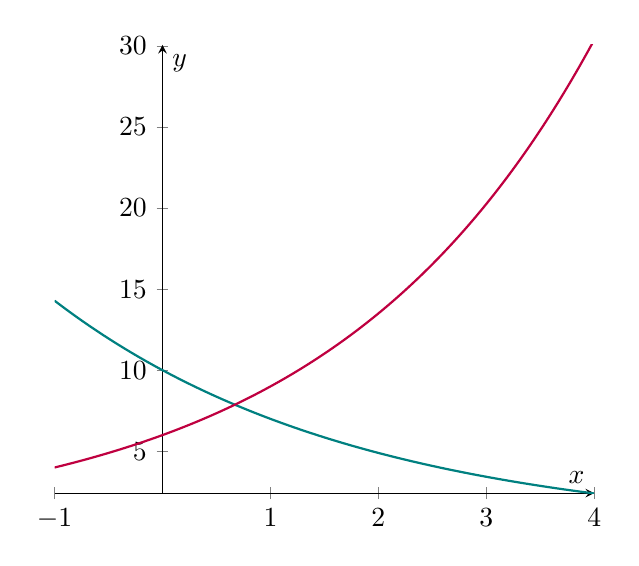
\begin{tikzpicture}
			\begin{axis}[axis lines = middle, xmin = -1, xmax = 4,
			xlabel = $x$, ylabel = $y$]
				\addplot[teal, thick, domain = -1:4, samples = 200] {10*0.7^x};
				\addplot[purple, thick, domain = -1:4, samples = 200] {6 * 1.5^x};
			\end{axis}
		\end{tikzpicture}
		\caption{Grafer for eksponentialfunktioner}
		\label{fig:eksp}
	\end{figure}
\end{exa}

Vi husker på, at $b$ i en eksponentialfunktion 
\begin{align*}
	f(x) = b \cdot a^x
\end{align*}
tilsvarer skæringen med y-aksen. Dette kan vi se, hvis vi indsætter $0$ på $x$' plads i forskriften
\begin{align*}
	f(0) = b \cdot a^0 = b \cdot 1 = b.
\end{align*}

\subsection*{Opgave 1}
For følgende eksponentialfunktioner aflæs da fremskrivningsfaktoren $a$ og begyndelsesværdien $b$.

\begin{align*}
	&a) \ f(x) = 6 \cdot 2^x    &&b) \  f(x) = 0.3 \cdot 1.5^x   \\
	&c) \ f(x) = 1.6 \cdot 0.7^x   &&d) \ f(x) = 200\cdot 0.1^x    \\  
\end{align*}

\subsection*{Opgave 2}

\begin{enumerate}[label = \roman*)]
	\item Bestem vækstraten for $f(x) = 2\cdot 1.6^x$.
	\item Bestem vækstraten for $f(x) = 5 \cdot 2.5^x$.
\end{enumerate}

\subsection*{Opgave 3}

Udfyld de tomme felter i følgende tabel. 

\begin{center}
	\begin{tabular}{c|c|c|c|c|c|c|}
		$f(x)$ & $1.1\cdot 1.2^x$ & \phantom{$1.1\cdot 1.2^x$} & \phantom{$1.1\cdot 1.2^x$} & \phantom{$1.1\cdot 1.2^x$}& $4.5 \cdot 2.1^x$ &\phantom{$1.1\cdot 1.2^x$}  \\
		\hline
		$a$ & & 2 & 1.7 & 4.7 & &  \\
		\hline
		$b$ & 1.1 & 10 & 22.5 & 15.2 & & 7.9 \\
		\hline
		$r$ & 0.2 & 1 & & & & 1.4 \\
	\end{tabular}
\end{center}

\subsection*{Opgave 4}
a) En eksponentialfunktion $f$ er givet ved
\begin{align*}
	f(x) = 6.7\cdot 1.3^x.
\end{align*}
\begin{enumerate}[label=\roman*)]
	\item Bestem $f(4)$.
	\item Bestem $f(-3)$.
\end{enumerate}

b) En eksponentialfunktion $g$ har begyndelsesværdi $7$ og fremskrivningsfaktor $0.7$.
\begin{enumerate}[label=\roman*)]
	\item Opskriv forskriften for $g$. 
	\item Bestem $g(7)$. 
\end{enumerate}


\subsection*{Opgave 5}

\begin{enumerate}[label= \roman*)]
	\item En eksponentialfunktion har en vækstrate på 0.5. Hvilken procentvis stigning vil 
	denne vækstrate tilsvare, når $x$ øges med 1?
	\item En eksponentialfunktion har en fremskrivningsfaktor på $1.1$. Hvilken procentvis 
	stigning vil denne fremskrivningsfaktor tilsvare, når $x$ øges med 1?
\end{enumerate}


\newpage

\subsection*{Opgave 6}
Følgende grafer for eksponentialfunktioner er givet.
\begin{enumerate}[label=\roman*)]
	\item Bestem $b$ for eksponentialfunktionerne
	\item Afgør, om $a$ er større eller mindre end 1.
\end{enumerate}
\begin{center}
	\resizebox{0.4\textwidth}{!}{
	\begin{tikzpicture}
		\begin{axis}[axis lines = middle, xmin = -1, xmax = 3,
		ytick = {1,2,...,10},
		ymin = -1,
		xlabel = $x$, ylabel = $y$]
			\addplot[teal, thick, domain = -1:4, samples = 200] {3*1.5^x};
		\end{axis}
	\end{tikzpicture}
	}
	\resizebox{0.4\textwidth}{!}{
	\begin{tikzpicture}
		\begin{axis}[axis lines = middle, xmin = -1, xmax = 4,
		ytick = {1,2,...,10},
		ymin = -1,
		xlabel = $x$, ylabel = $y$]
			\addplot[teal, thick, domain = -1:4, samples = 200] {6 * 0.6^x};
		\end{axis}
	\end{tikzpicture}
	}
	\resizebox{0.4\textwidth}{!}{
	\begin{tikzpicture}
		\begin{axis}[axis lines = middle, xmin = -0.2, xmax = 4,
		ytick = {1,2,...,12},
		ymin = -1,
		xlabel = $x$, ylabel = $y$]
			\addplot[teal, thick, domain = -0.2:4, samples = 200] {9 * 0.2^x};
		\end{axis}
	\end{tikzpicture}
	}
	\resizebox{0.4\textwidth}{!}{
	\begin{tikzpicture}
		\begin{axis}[axis lines = middle, xmin = -1, xmax = 3,
		ytick = {1,2,...,16},
		ymin = -1,
		xlabel = $x$, ylabel = $y$]
			\addplot[teal, thick, domain = -1:3, samples = 200] {2 * 2^x};
		\end{axis}
	\end{tikzpicture}
	}
\end{center}


\subsection*{Opgave 7}
Hver gang vi folder et stykke papir, så vil antallet af papirlag fordobles. Antallet af lag kan beskrives af en eksponentialfunktion 
\begin{align*}
	f(x) = b\cdot a^x.
\end{align*}
\begin{enumerate}[label=\roman*)]
	\item Hvad er begyndelsesværdien og fremskrivningsfaktoren for $f$?
	\item Hvor mange lag har et stykke papir, hvis det er foldet 7 gange?
	\item Forestil dig, at du kan folde papiret lige så mange gange du har lyst. Hvor tykt er
	papiret, hvis du har foldet det 25 gange?
 	\item Hvis ét lag papir er 0.1mm tykt, hvor tykt er dette stykke foldede papir?
	\item Hvor mange gange skal vi folde papiret, for at det bliver 1km tykt?
\end{enumerate}


\subsection*{Opgave 8}
\begin{enumerate}[label=\roman*)]
\item En bakteriekoloni indeholder til tid $t=0$ $B_0 = 100.000$ bakterier. En bakterie deler sig i gennemsnit 1 gang per 4. time, og bakteriekolonien har ubegrænset plads. Beskriv antallet af bakterier som funktion af tiden i timer. Hvor mange bakterier er der i kolonien efter et døgn? Hvornår er der 1 mia. $(10^9)$ bakterier i kolonien?
\item Et glas vand stilles i et rum, og temperaturen i vandet antages at kunne beskrives ved
\begin{align*}
H(t) = 70\cdot(0.97)^t,
\end{align*}
hvor $H(t)$ beskriver temperaturen i grader celcius og $t$ betegner tiden i minutter. Hvor varmt er vandet, når det stilles ind i rummet? Hvor varmt er det efter 5 minutter? Hvor varmt er der i rummet i følge modellen. 
\end{enumerate}

\subsection*{Opgave 9}
\begin{enumerate}[label=\roman*)]
\item Bevis, at hvis vi øger $x$ med 2 i en eksponentialfunktion $f(x)$, så tilsvarer dette at øge $f(x)$ med en faktor $a^2$. Hvad hvis vi øger $x$ med $3$?
\item Bevis, at hvis vi øger $x$ med $n$ i en eksponentialfunktion $f(x)$, så tilsvarer dette at øge $f(x)$ med en faktor $a^n$.
\end{enumerate}
